\documentclass[../Carre_nights.tex]{subfiles}

\begin{document}

\section{n0180}
\textbf{\Large{The tale of Kamar al-Zaman and princess Budur}} \\

\begin{figure}[ht]
\centering
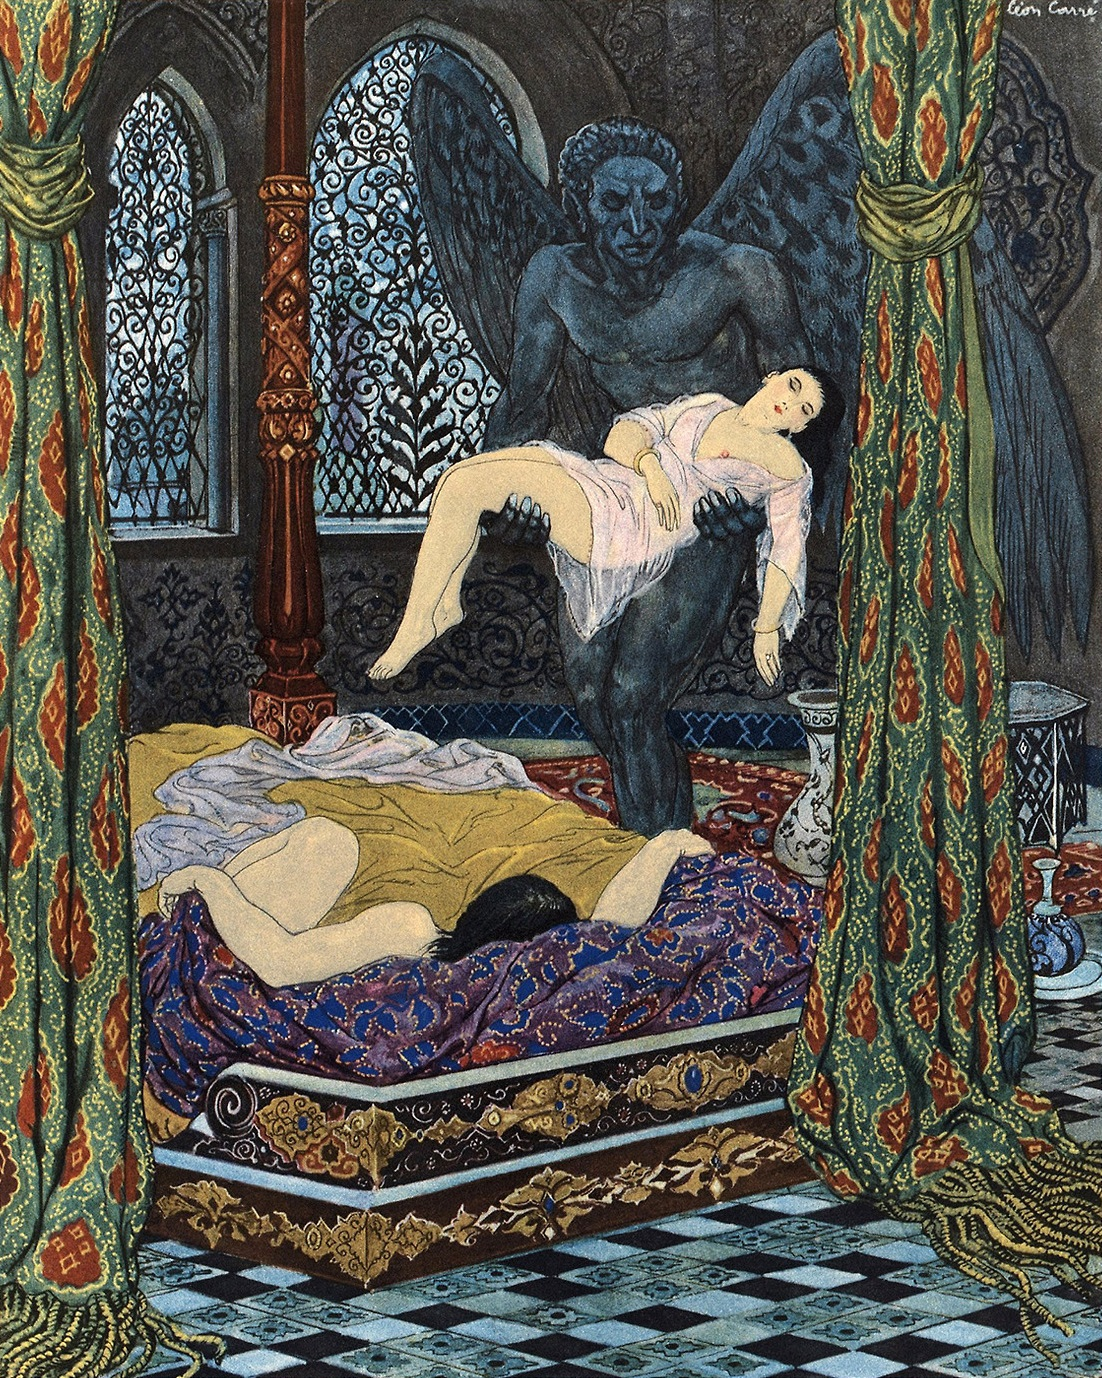
\includegraphics[height=\figsize]{illustrations/volume_3/T03, n0180 - Histoire de la princesse Boudour.jpg}
\end{figure}

\textit{\\
"...l’éfrit Dahnasch, avec des précautions infinies, déposa doucement la princesse sur le lit, et lui enleva sa chemise."} \\
—T03, n0180 - Histoire de la princesse Boudour \\~\\
\textit{"...Dahnash, with infinite precaution, laid the princess on the bed and took off her chemise."} \\
—V02, n0180 - The tale of Kamar al-Zaman and princess Budur

\newpage

\section{n0188}
\textbf{\Large{The tale of Kamar al-Zaman and princess Budur}} \\

\begin{figure}[ht]
\centering
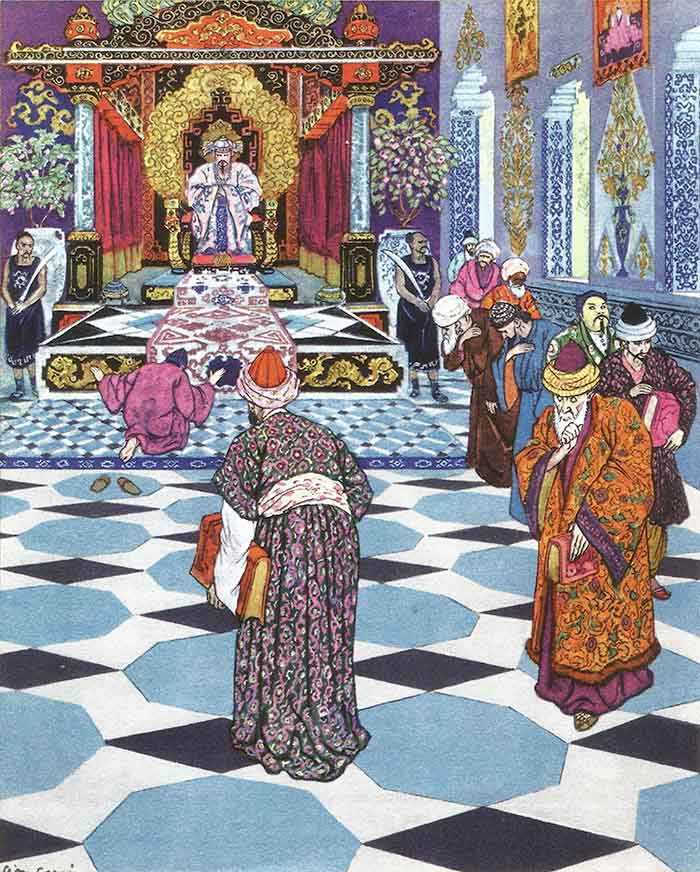
\includegraphics[height=\figsize]{illustrations/volume_3/T03, n0188 - Histoire de la princesse Boudour.jpg}
\end{figure}

\textit{\\
"Il assembla donc dans son palais tous les savants de son royaume, les médecins, les astrologues, les magiciens, les hommes versés dans les livres anciens, et les droguistes..."} \\
—T03, n0188 - Histoire de la princesse Boudour \\~\\
\textit{"He called together all the learned men of his kingdom, the doctors, astrologers, chemists, and those versed in the books of old..."} \\
—V02, n0188 - The tale of Kamar al-Zaman and princess Budur

\newpage

\section{n0222}
\textbf{\Large{The tale of Kamar al-Zaman and princess Budur}} \\

\begin{figure}[ht]
\centering
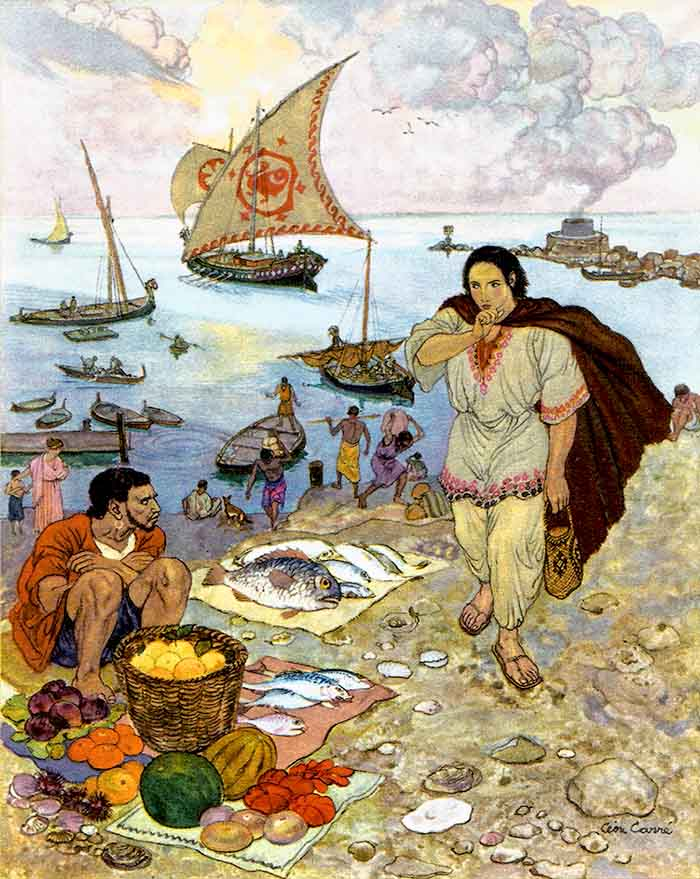
\includegraphics[height=\figsize]{illustrations/volume_3/T03, n0222 - Histoire de la princesse Boudour.jpg}
\end{figure}

\textit{\\
"Il acheta quelques provisions, ferma la porte du jardin, prit la clef avec lui, et courut en hâte au port, alors que le soleil était déjà bien haut ; mais ce fut pour voir le navire, toutes voiles dehors, emporté par le vent favorable vers la haute mer."} \\
—T03, n0222 - Histoire de la princesse Boudour \\~\\
\textit{"He collected provision for the journey, locked the gate of the garden, and ran in haste to the harbour; the sun was already high and he saw the ship that should have carried him making, with all sails set before a favourable wind, for the open sea."} \\
—V02, n0222 - The tale of Kamar al-Zaman and princess Budur

\newpage

\section{n0238}
\textbf{\Large{The tale of Happy-Handsome and Happy-Fair}} \\

\begin{figure}[ht]
\centering
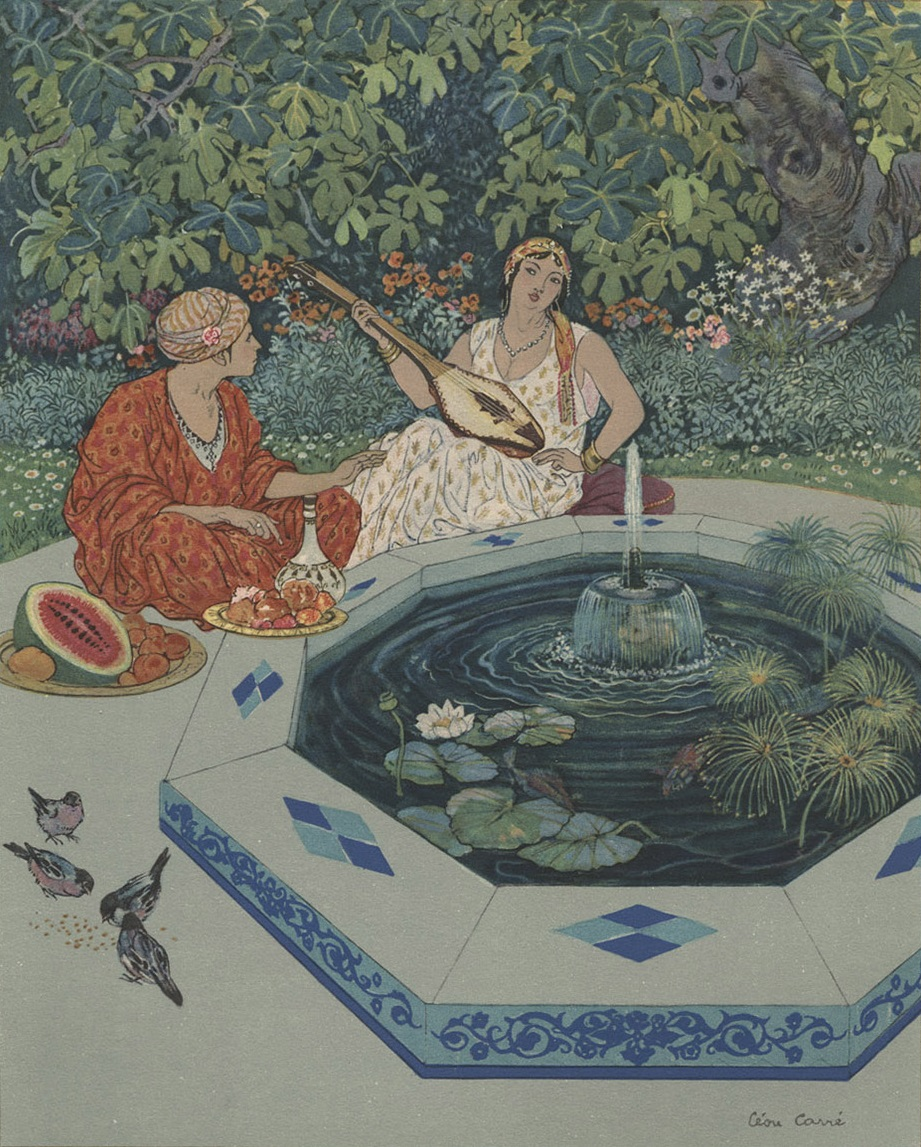
\includegraphics[height=\figsize]{illustrations/volume_3/T03, n0238 - Histoire de Bel-Heureux et de Belle-Heureuse.jpg}
\end{figure}

\textit{\\
"...que de fois Bel-Heureux et son esclave Belle-Heureuse ne venaient-ils pas, aux heures chaudes, s’asseoir dans leur jardin, sur le marbre nu, autour du bassin, où la fraîcheur de l’eau et de la pierre les pénétrait de délices."} \\
—T03, n0238 - Histoire de Bel-Heureux et de Belle-Heureuse \\~\\
\textit{"Happy-Handsome and Happy-Fair spent the warm hours of each day sitting in their garden, on the naked marble of the fish-pond, refreshed by the cool water and the cool stone."} \\
—V02, n0238 - The tale of Happy-Handsome and Happy-Fair

\newpage

\section{n0246}
\textbf{\Large{The tale of Happy-Handsome and Happy-Fair}} \\

\begin{figure}[ht]
\centering
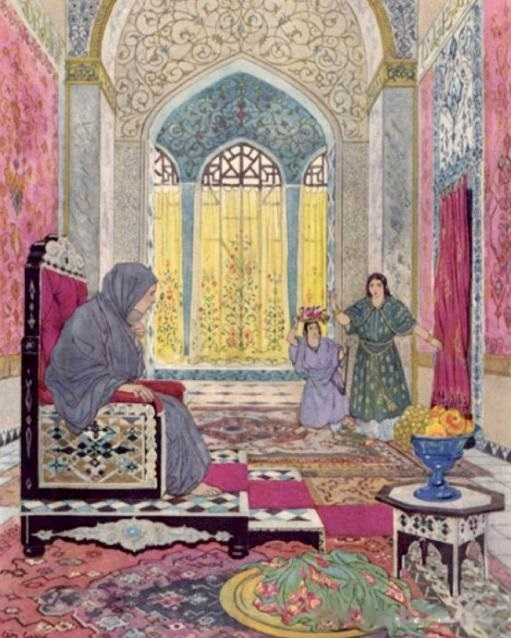
\includegraphics[height=\figsize]{illustrations/volume_3/T03, n0246 - Histoire de Bel-Heureux et de Belle-Heureuse.jpg}
\end{figure}

\textit{\\
"...il vit entrer, par l’une des portes latérales, une jeune femme à l’aspect royal, habillée seulement de ses vêtements d’intérieur, sans voile sur le visage ou foulard sur les cheveux. Et elle était suivie d’une esclave mignonne, les pieds nus, qui portait sur la tête des fleurs et tenait à la main un luth en bois de sycomore."} \\
—T03, n0246 - Histoire de Bel-Heureux et de Belle-Heureuse \\~\\
\textit{"...he saw a young woman with a royal look enter by one of the side doors. She was dressed only in house garments, so that her face and hair might be seen; and was followed by a delicious little slave with naked feet, who was crowned with flowers and carried a lute of sycamore-wood in her hand."} \\
—V02, n0246 - The tale of Happy-Handsome and Happy-Fair

\newpage

\section{n0259}
\textbf{\Large{The tale of Ala al-Din Abu Shamat}} \\

\begin{figure}[ht]
\centering
\includegraphics[height=\figsize]{illustrations/volume_3/T03, n0259 - Histoire de Grain-de-beauté.jpg}
\end{figure}

\textit{\\
"...il mangea un morceau ; puis, les esclaves partis se coucher, il sortit de la tente et s’éloigna un peu dans la vallée et alla s’asseoir sous un arbre au clair de lune."} \\
—T03, n0259 - Histoire de Grain-de-beauté \\~\\
\textit{"Abu Shamat ate a light meal and then, when the slaves had lain down to sleep, left his tent and, walking up the valley for a little way, sat down under a tree in the moonlight."} \\
—V02, n0259 - The tale of Ala al-Din Abu Shamat

\newpage

\section{n0269}
\textbf{\Large{The tale of Ala al-Din Abu Shamat}} \\

\begin{figure}[ht]
\centering
\includegraphics[height=\figsize]{illustrations/volume_3/T03, n0269 - Histoire de Grain-de-beauté.jpg}
\end{figure}

\textit{\\
"...le lit se souleva de lui-même en l’air, sans secousses, monta jusqu’à la coupole, sortit par la grande fenêtre, et, plus rapide que le plus rapide d’entre les oiseaux, il fendit l’espace avec une régularité merveilleuse..."} \\
—T03, n0269 - Histoire de Grain-de-beauté \\~\\
\textit{"...the bed rose in the air, without any jolting, and, going out by the great window in the dome, began to sail through the air more quickly than a bird, but with an easy and riding motion."} \\
—V02, n0269 - The tale of Ala al-Din Abu Shamat

\newpage

\section{n0272}
\textbf{\Large{The tale of Sympathy the learned}} \\

\begin{figure}[ht]
\centering
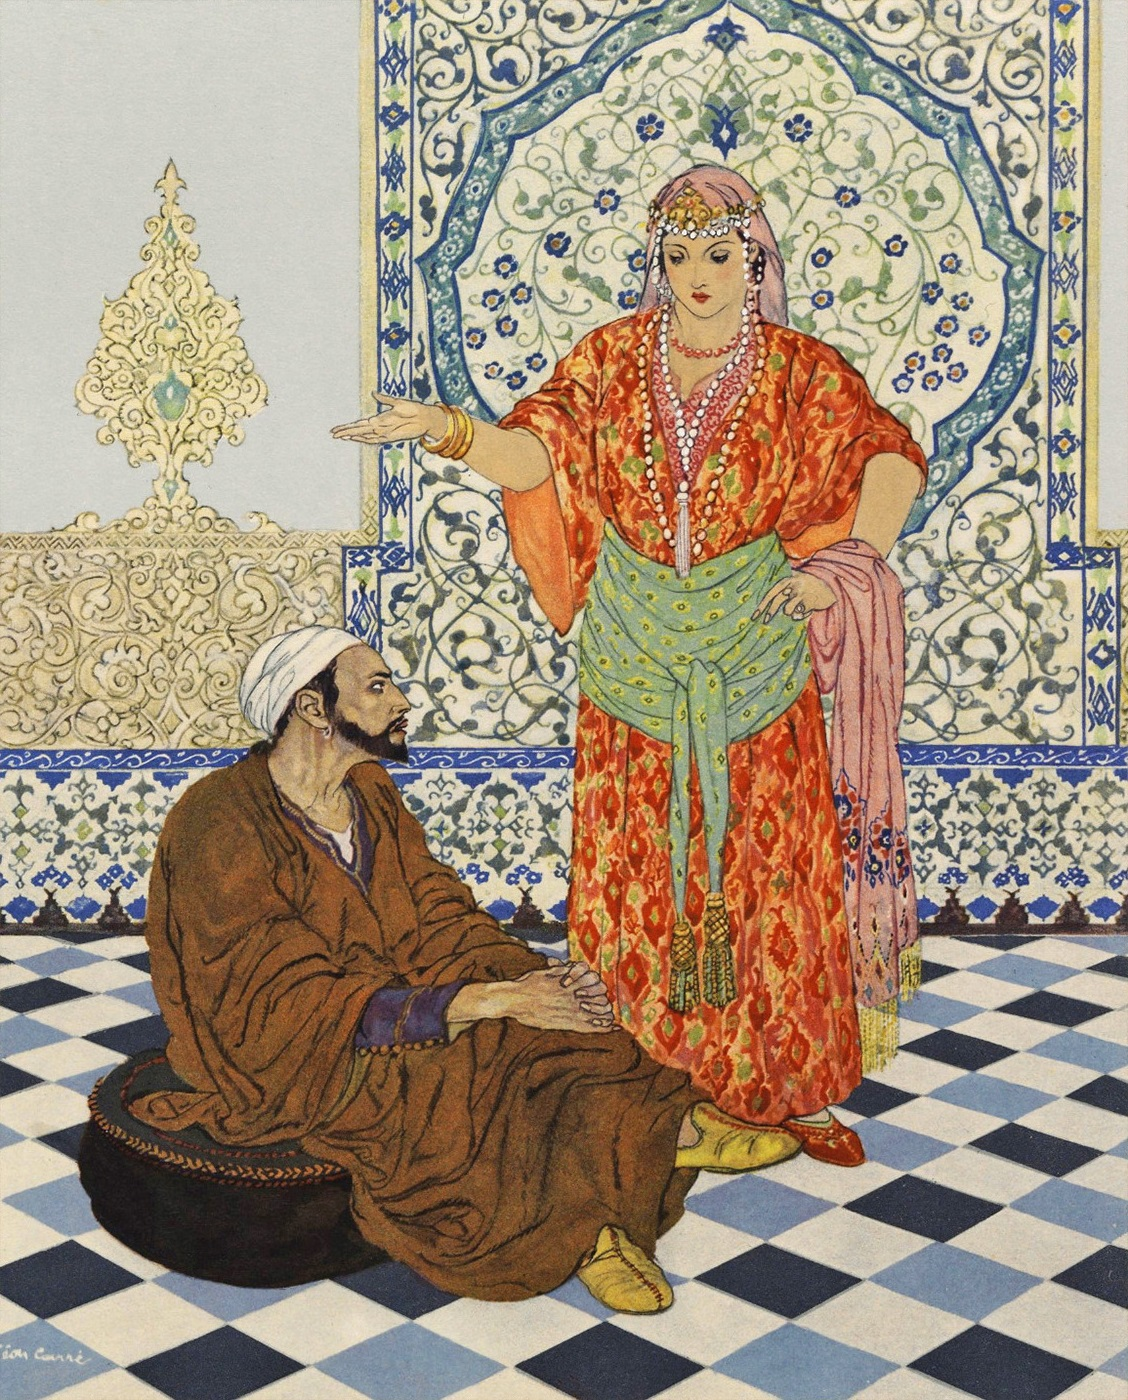
\includegraphics[height=\figsize]{illustrations/volume_3/T03, n0272 - Histoire de la docte Sympathie.jpg}
\end{figure}

\textit{\\
"Elle se para de ses belles robes et se présenta à son maître avec, sur les lèvres, un sourire de bon augure, en lui disant : « Allah va faire cesser tes tribulations par mon entremise."} \\
—T03, n0272 - Histoire de la docte Sympathie \\~\\
\textit{"She put on the rest of her jewels and those robes which remained most fit to be seen; then she went to her master and said with an encouraging smile: 'Allah will put an end to your misfortunes by my help."} \\
—V02, n0271 - The tale of Sympathy the learned

\newpage

\section{n0287}
\textbf{\Large{An adventure of the poet Abu Nuwas}} \\

\begin{figure}[ht]
\centering
\includegraphics[height=\figsize]{illustrations/volume_3/T03, n0287 - Aventures du poète Abou-Nowas.jpg}
\end{figure}

\textit{\\
"...s’avançant vers le lit, il en releva les rideaux. Et il resta émerveillé de la beauté endormie qui s’offrait à son regard. C’était une jeune esclave, la lune dans son plein, et dont la chevelure éployée était le seul voile."} \\
—T03, n0287 - Aventures du poète Abou-Nowas \\~\\
\textit{"...he lifted the curtains of the bed and stood stock-still with amazement at the sleeping beauty of a slave who lay there, as fair as the full moon, covered for sole garment with her fallen hair."} \\
—V02, n0287 - An adventure of the poet Abu Nuwas

\newpage

\section{n0292}
\textbf{\Large{The tale of Sindbad the sailor [The first voyage]}} \\

\begin{figure}[ht]
\centering
\includegraphics[height=\figsize]{illustrations/volume_3/T03, n0292 - Sindbad le marin [La première histoire].jpg}
\end{figure}

\textit{\\
"...nous vîmes apparaître à l’avant du navire le capitaine qui, d’une voix terrible et avec des gestes effrayants, nous cria : « Ô passagers, sauvez-vous ! Hâtez-vous ! Remontez vite à bord ! Lâchez tout ! Abandonnez vos effets à terre et sauvez vos âmes ! Fuyez l’abîme ! Courez vite ! Car l’île n’est point une île ! C’est une baleine gigantesque !"} \\
—T03, n0292 - Sindbad le marin [La première histoire] \\~\\
\textit{"...we saw the captain appear in the bows of his ship and heard him cry in an agonized voice with wild gesturings: 'Save yourselves! Come aboard for your lives! That is no island but a gigantic whale!"} \\
—V02, n0292 - The tale of Sindbad the sailor [The first voyage]

\newpage

\section{n0296}
\textbf{\Large{The tale of Sindbad the sailor [The second voyage]}} \\

\begin{figure}[ht]
\centering
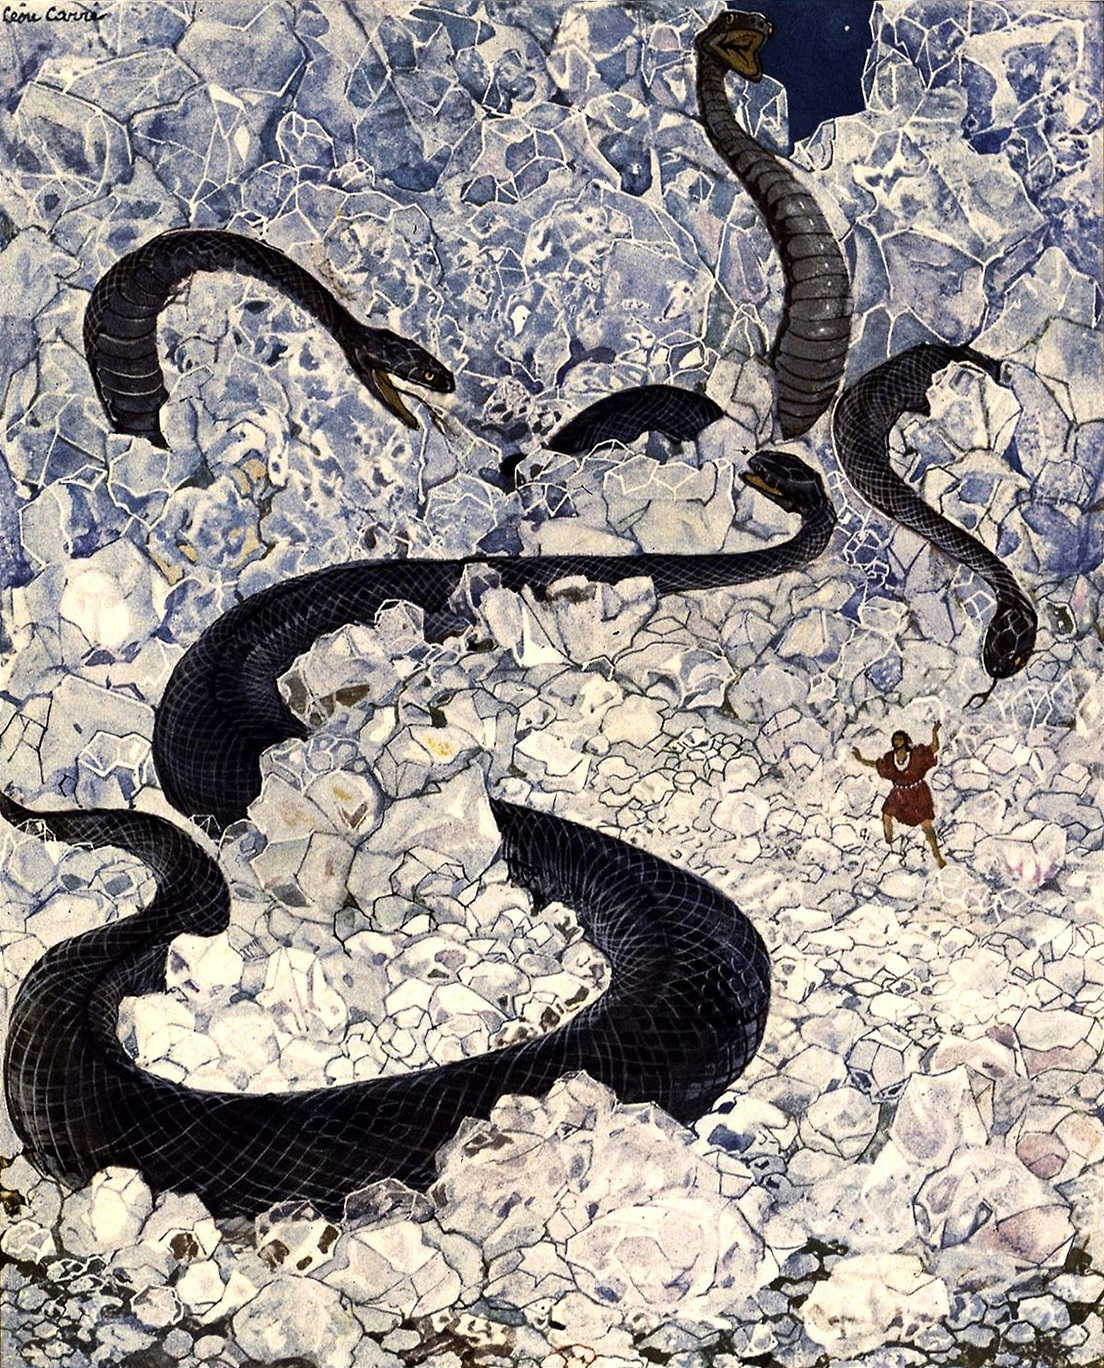
\includegraphics[height=\figsize]{illustrations/volume_3/T03, n0296 - Sindbad le marin [La seconde histoire].jpg}
\end{figure}

\textit{\\
"Au milieu des roches de diamant, je vis circuler les gardiens qui étaient des serpents noirs en quantité innombrable, plus gros et plus grands que des palmiers, et qui pouvaient certainement en- gloutir, chacun d’eux, un buffle ou un éléphant."} \\
—T03, n0296 - Sindbad le marin [La seconde histoire] \\~\\
\textit{"The guardians of the diamond rocks were moving about their treasure, innumerable black snakes, thicker and longer than palm-trees, each one of which could have swallowed a large elephant."} \\
—V02, n0296 - The tale of Sindbad the sailor [The second voyage]

\newpage

\section{n0316}
\textbf{\Large{The tale of Zumurrud the beautiful}} \\

\begin{figure}[ht]
\centering
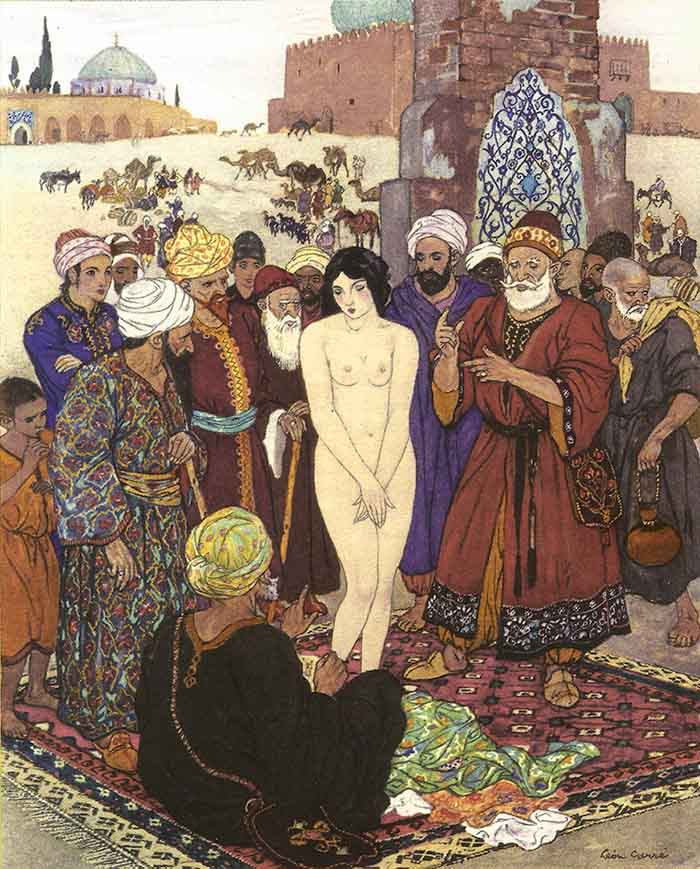
\includegraphics[height=\figsize]{illustrations/volume_3/T03, n0316 - Histoire de la belle Zoumouroud.jpg}
\end{figure}

\textit{\\
"...il vit une grande foule rassemblée. Il fut tenté de s’en approcher, pour juger de ce qui se passait, et il vit, au milieu du cercle formé par les marchands, par les courtiers et les acheteur une jeune esclave blanche d’une délicieuse tournure..."} \\
—T03, n0316 - Histoire de la belle Zoumouroud \\~\\
\textit{"...he saw a crowd collected in a circle. He went towards these people to see what was happening and saw, in the centre of a group of brokers, merchants and purchasers, a young white slave of elegant and delightful appearance."} \\
—V02, n0316 - The tale of Zumurrud the beautiful

\newpage

\section{n0331}
\textbf{\Large{The tale of Zumurrud the beautiful}} \\

\begin{figure}[ht]
\centering
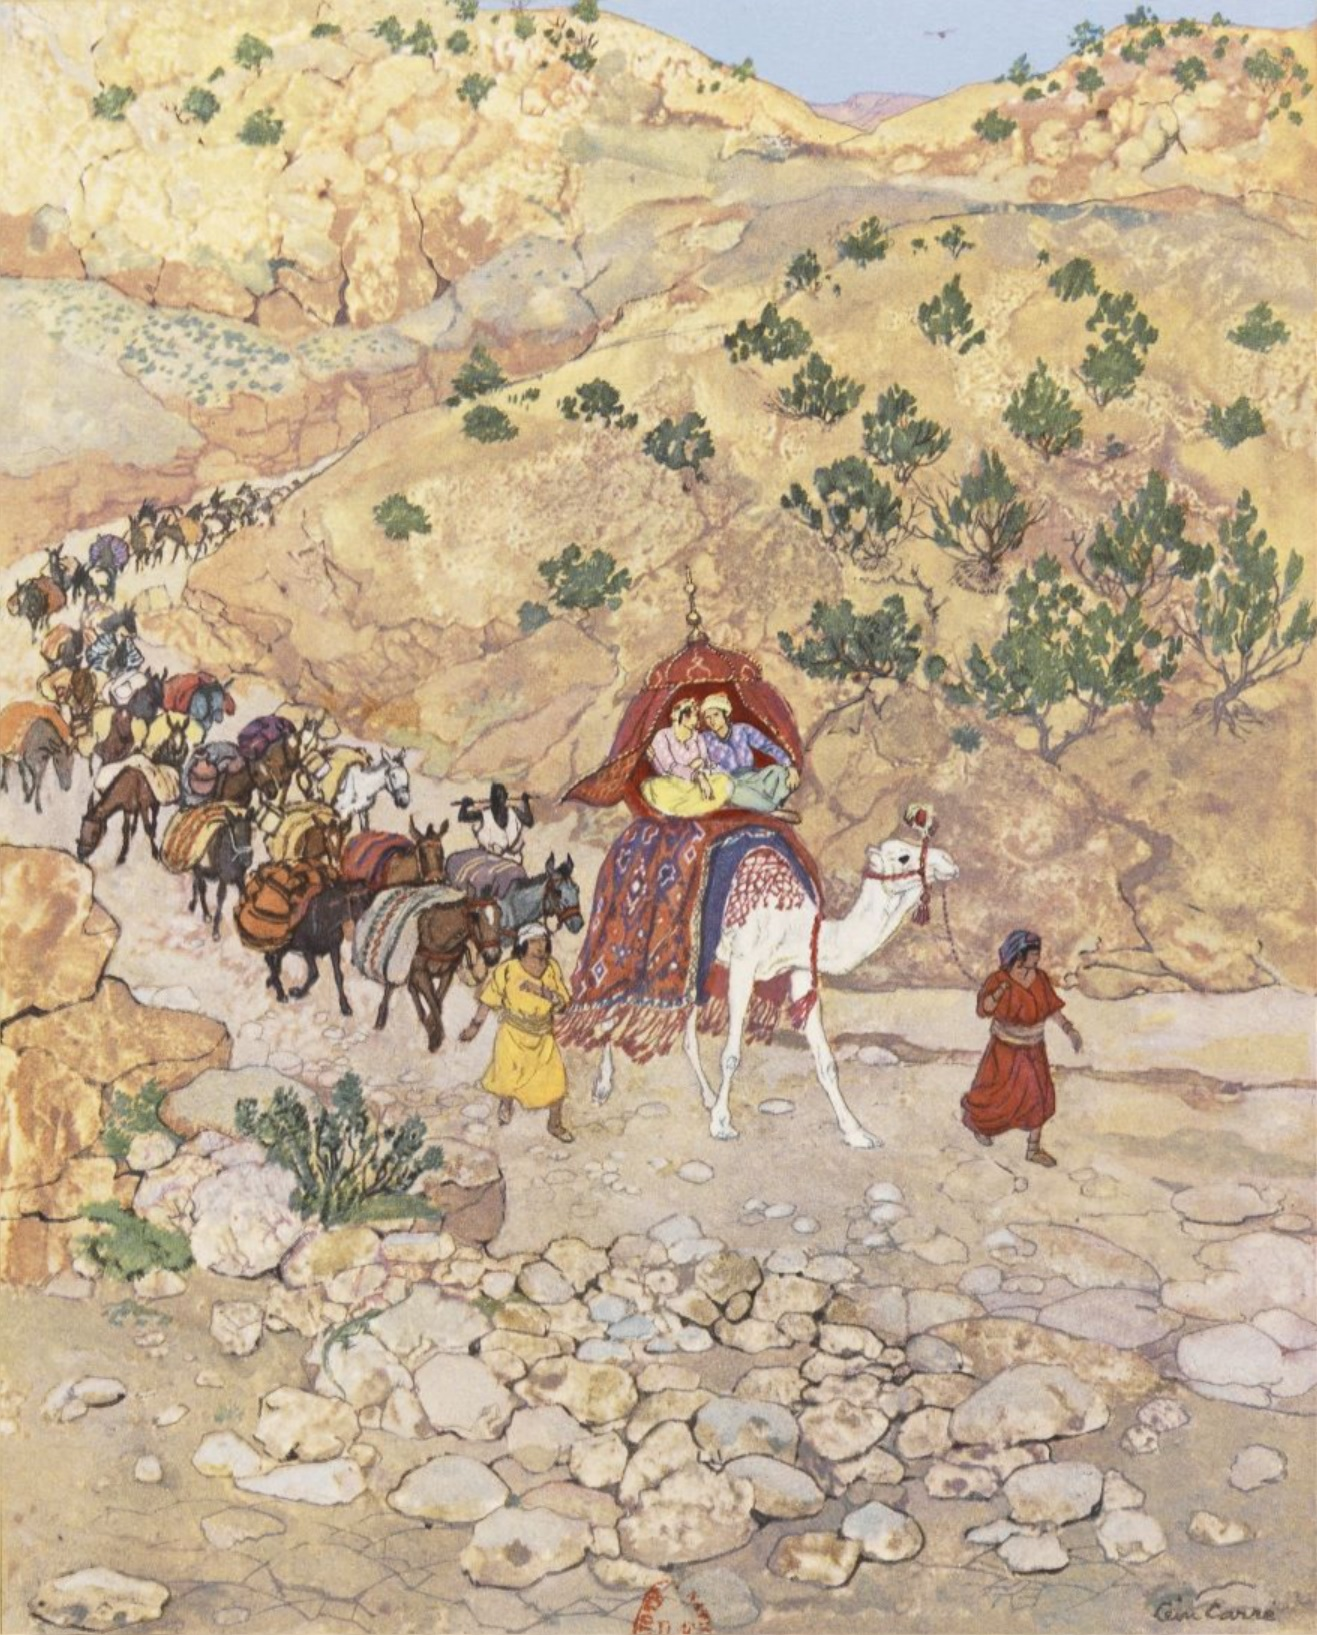
\includegraphics[height=\figsize]{illustrations/volume_3/T03, n0331 - Histoire de la belle Zoumouroud.jpg}
\end{figure}

\textit{\\
"...sitôt tout cela prêt, Zoumourroud et Alischar montèrent dans un palanquin de velours porté par un dromadaire, et, suivis des deux petits eunuques seulement, ils retournèrent au Khorassân..."} \\
—T03, n0331 - Histoire de la belle Zoumouroud \\~\\
\textit{"When all was in readiness, Zumurrud and Ali Shar got up into a velvet and brocaded palanquin, carried by a dromedary, and, accompanied only by the two little eunuchs, journeyed to the land of Khurasan..."} \\
—V02, n0331 - The tale of Zumurrud the beautiful

\newpage

\section{n0332}
\textbf{\Large{The tale of the six different coloured girls}} \\

\begin{figure}[ht]
\centering
\includegraphics[height=\figsize]{illustrations/volume_3/T03, n0332 - Histoire des six adolescentes aux couleurs différentes.jpg}
\end{figure}

\textit{\\
"...un jour, Ali El-Yamani, heureux de la quiétude goûtée dans la délectable Baghdad, et se sentant dans des dispositions d’esprit meilleures encore que d’habitude, invita ses six esclaves à la fois à venir dans la salle de réunion lui tenir compagnie et passer le temps à boire, à s’entretenir et à chanter avec lui."} \\
—T03, n0332 - Histoire des six adolescentes aux couleurs différentes \\~\\
\textit{"...one day, when Ali al-Yaman felt in better spirits than usual, owing to the delectable peace which he experienced in our city, he invited his six slaves to come together to keep him company, to drink, to talk, and to sing with him."} \\
—V02, n0332 - The tale of the six different coloured girls

\newpage

\section{n0343}
\textbf{\Large{The extraordinary tale of the city of brass}} \\

\begin{figure}[ht]
\centering
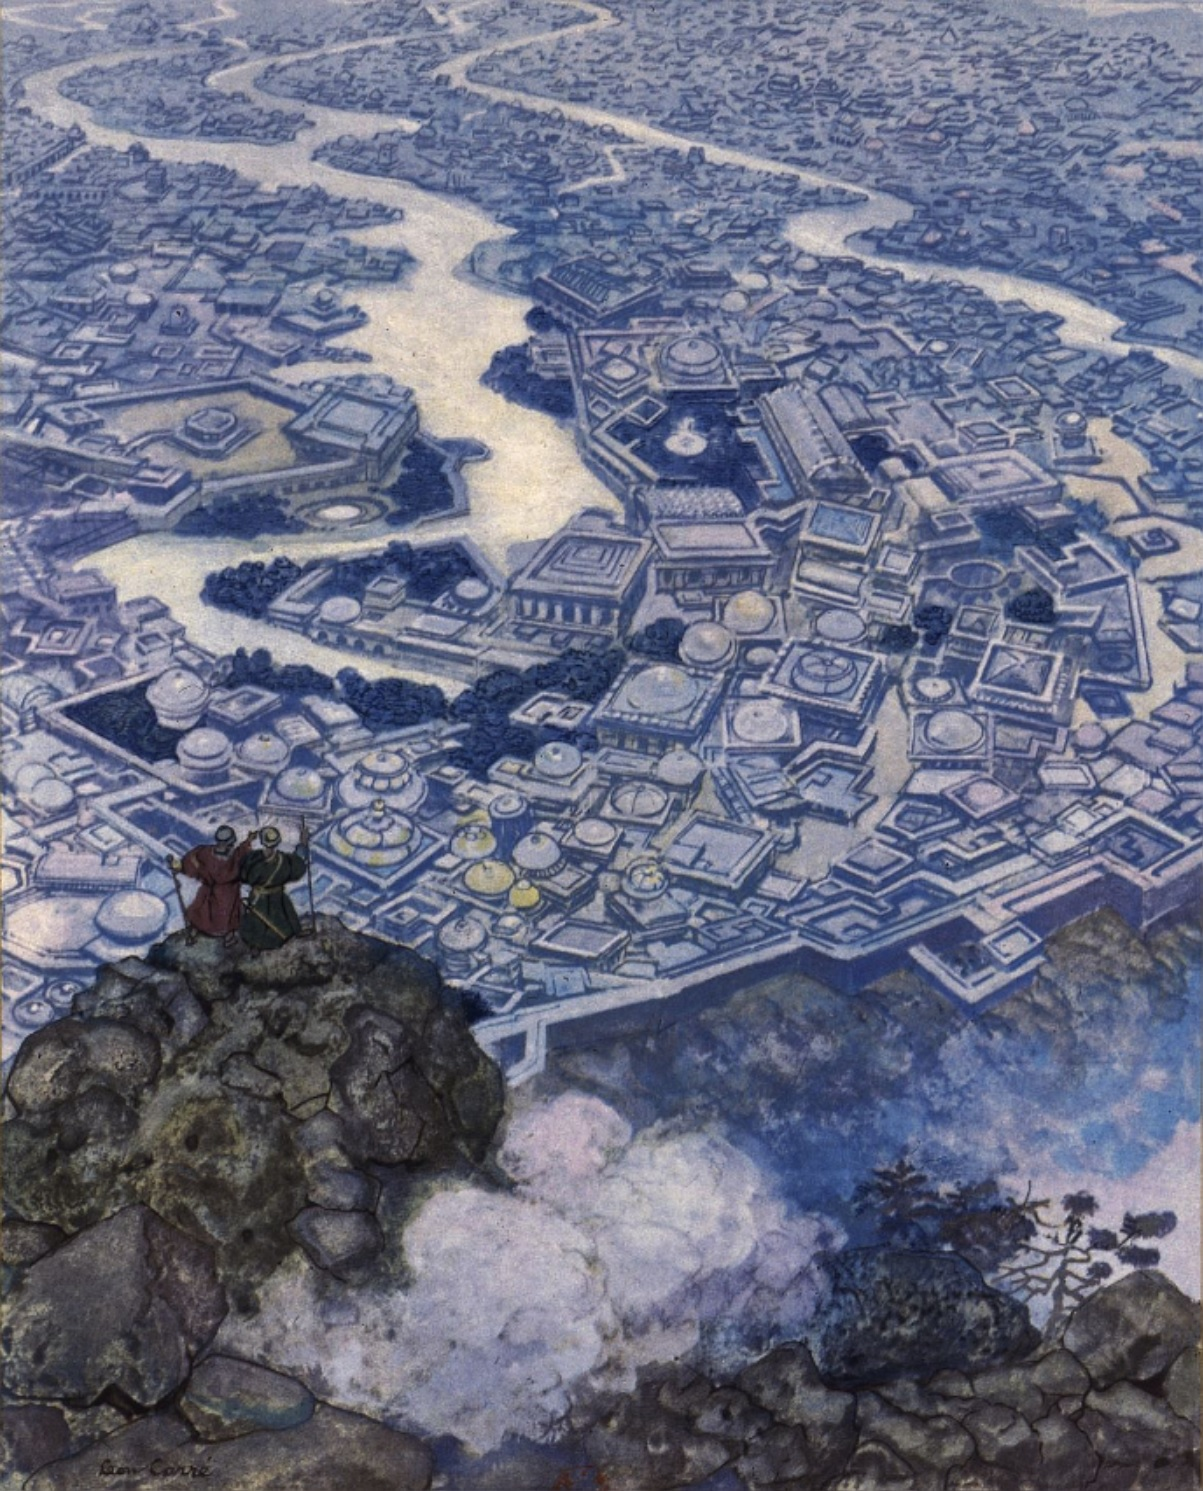
\includegraphics[height=\figsize]{illustrations/volume_3/T03, n0343 - Histoire de la ville d'airain.jpg}
\end{figure}

\textit{\\
"...soudain la lueur à l’Orient se fit plus vive, et sur le sommet de la montagne la lune magnifique s’élança et, d’un clignement, illumina le ciel et la terre. Et à leurs pieds un spectacle se déroula qui les fit s’arrêter de respirer. Ils dominaient une ville de songe."} \\
—T03, n0343 - Histoire de la ville d'airain \\~\\
\textit{"...suddenly the light in the east grew greater and the splendid moon swam from behind the top of a mountain and lighted earth and sky at once with the sparkling of her eyes. Then at their feet unrolled a sight which made them hold their breath. They were looking down upon a city of dream."} \\
—V02, n0343 - The extraordinary tale of the city of brass

\end{document}